In this section, we conduct a preliminary empirical study of SCOPE using the TextCraft environment. 


\textbf{Dataset and Network Architecture.} To simulate suboptimal trajectories resembling those of human players, we generate 500K rollouts, reserving 1K each for validation and testing. The objective is to obtain diverse trajectories that generally progress toward the target goal in the TextCraft environment while including occasional suboptimal actions to mimic human-like exploration. Starting from a given state space (defined by available crafting commands) and a target goal item, we construct the recipe tree, derive the optimal crafting sequence, and inject random actions at a 10\% rate to introduce variability. The resulting trajectories blend optimal and noisy transitions, producing behaviour that closely resembles human demonstrations.  

Although the employee and manager agents differ in their input-output formats, all signals are converted to text for unified processing, enabling both to share a variational sequence-to-sequence architecture (see \Cref{appx:model_arch} for details). The hyperparameter settings are provided in \Cref{appx:hyperparameter}. 

\begin{table*}
\centering
\caption{Success rates for crafting ace items in TextCraft. \textbf{Top:} ADaPT \citep{PrasadKHCSBK2024} is a hierarchical agent that uses a GPT-3.5-based planner \citep{BrownMRSSKD2020}. \textbf{Bottom:} Ablation results. SCOPE (hand-engineered-subgoal) replaces LLM-generated subgoals with manually constructed, interpretable ones. SCOPE (without manager RL-finetuning) removes the manager-level RL stage.
}
\label{tab:performance}
\begin{tabular}{l c c}
\toprule
\textbf{Setting} & \textbf{Success Rate} & \textbf{\# Parameters} \\
\midrule
ADaPT \citep{PrasadKHCSBK2024} & 0.52 & 175B \\
SCOPE (\textbf{ours})  & 0.56 & 11.04M \\
\midrule
SCOPE (hand-engineered-subgoal) & 0.58 & 11.04M \\
SCOPE (without manager RL-finetuning) & 0.24 & 11.04M \\
\bottomrule
\end{tabular}
\vspace{1em}  
\end{table*}



\begin{table*}[t]
    \centering
    \caption{Success rates for crafting ace items in TextCraft for ADaPT \citep{PrasadKHCSBK2024} with different backends. The original implementation uses GPT-3.5 \citep{BrownMRSSKD2020} as the backend.}
    \label{tab:backend-success}
%    \begin{tabular}{lcc}
%        \toprule
%        \textbf{Backend} & \textbf{Success Rate} & \textbf{\# Parameters} \\
%        \midrule
%        GPT-4o            & 0.58  & 1.8T$^{*}$ \\
%        Mistral Small 3  & 0.58   & 24B \\
%        SCOPE            & 0.56   & 11.04M \\
%        GPT-3.5           & 0.52   & 175B \\
%        GPT-4o mini       & 0.43  & 8B$^{*}$ \\
%        DeepSeek-R1-Distill-Qwen-32B           & 0.13   & 32B \\
%        Claude-3 Haiku   & 0.00      & 20B$^{*}$ \\
%        \bottomrule
%    \end{tabular}

\resizebox{\textwidth}{!}{
    \begin{tabular}{lccc}
    \toprule
    \textbf{Backend} & \textbf{Success Rate} & \textbf{\# Parameters} & \textbf{Open Weight?} \\
    \midrule
    GPT-4o \citep{OpenAI2024}                         & 0.58 & 1.8T$^{*}$ & No  \\
    Mistral Small 3 \citep{mistral_small3_2025}       & 0.58 & 24B        & Yes \\
    SCOPE (\textbf{ours})                          & 0.56 & 11.04M     & - \\
    GPT-3.5 \citep{BrownMRSSKD2020}                        & 0.52 & 175B       & No  \\
    GPT-4o mini \citep{OpenAI2024}                    & 0.43 & 8B$^{*}$   & No  \\
    DeepSeek-R1-Distill-Qwen-32B \citep{DeepSeek-AI2025}    & 0.13 & 32B        & Yes \\
    Claude-3 Haiku \citep{anthropic_claude3_2024}                 & 0.00 & 20B$^{*}$  & No  \\
    \bottomrule
\end{tabular} 
}%  
    \vspace{0.3em}
    {\footnotesize $^{*}$ Rough estimates based on publicly discussed or widely believed parameter counts.}
\end{table*}



%\textbf{Effectiveness of the Proposed Method.} 

\subsection{Performance Comparison}
As shown in \Cref{tab:performance}, ADaPT \citep{PrasadKHCSBK2024} is a hierarchical framework that relies on an LLM-based planner with a GPT-3.5 backend \citep{BrownMRSSKD2020}, and it achieves a success rate of 0.52. In comparison, SCOPE attains an ultimate-goal success rate of 0.56. This shows that a one-time LLM initialization, followed by RL fine-tuning, can outperform methods that depend on LLM inference throughout execution.
The reduced model size also leads to substantially lower inference cost and latency. In particular, SCOPE agent completes the game in an average of 3.0 seconds on an NVIDIA A10 GPU, whereas ADaPT requires 164.4 seconds when using a GPT-3.5 backend accessed via the OpenAI API under ideal network conditions.


In addition to the original ADaPT implementation based on GPT-3.5 \citep{BrownMRSSKD2020}, we also report results using a broader selection of backends in \Cref{tab:backend-success}. The table compares ADaPT with a range of LLM backends that vary in size and openness. GPT-4o is a large proprietary model developed by OpenAI~(\citeyear{OpenAI2024}), and GPT-4o mini is a smaller, more cost-efficient variant intended to reduce latency and compute while retaining much of GPT-4o’s capability. Claude-3 Haiku \citep{anthropic_claude3_2024} is Anthropic’s lightweight model, designed to answer many requests quickly and reliably under tight latency or budget constraints. On the open-weight side, Mistral Small 3 \citep{mistral_small3_2025} is a 24B-parameter model in the ``small'' LLM category (below 70B) that delivers performance comparable to substantially larger models. DeepSeek-R1-Distill-Qwen-32B \citep{DeepSeek-AI2025} is a mid-sized reasoning model distilled from DeepSeek-R1 based on Qwen2.5 \citep{Qwen2024}. It achieves competitive or superior results to OpenAI o1-mini \citep{OpenAI2024-o1} on a range of benchmarks, representing a strong open-weight option in the dense-model regime. While using these more advanced backends improves ADaPT’s performance, SCOPE remains highly competitive: with only 11.04M parameters, it attains a success rate of 0.56, coming very close to the performance of GPT-4o and Mistral Small 3 (both 0.58 with tens of billions to trillions of parameters) and outperforming GPT-4o mini, DeepSeek-R1-Distill-Qwen-32B, and Claude-3 Haiku. This underscores how parameter-efficient SCOPE is compared to both closed and open-weight alternatives.

\subsection{Impact of Suboptimal Subgoals on Performance} 
\label{sec:impact_subopt_subgoal_performance}

To better understand how much performance degradation results from suboptimal subgoals, in \Cref{fig:subgoal_seq}, we compare the subgoals produced by \(f_{\text{dc}}\) with those generated through a hand-engineered, more interpretable procedure. In the hand-engineered version, each subgoal is defined as the inventory state immediately after an intermediate item is crafted in a demonstration trajectory. The subgoal is considered achieved once the agent's inventory contains at least the same items as those target state. By sequentially completing these preset subgoals, the agent eventually crafts the ace item, as the final subgoal contains the ace item to be crafted.  Note that while such hand-crafted and interpretable subgoal decomposition is feasible for this simple TextCraft environment, in more complex settings, LLM-generated subgoal decomposition may be the only practical option.


In contrast, the subgoals proposed by \(f_{\text{dc}}\) are far less interpretable, and it is unclear how the employee agent should leverage them as effective guidance for crafting the ace item. Interestingly, despite their limited explainability and potential suboptimality, these LLM-generated subgoals still provide sufficient structure for the hierarchical agent to learn and achieve strong performance. In particular, as shown in \Cref{tab:performance}, using fully explainable, hand-engineered subgoals improves the success rate by only 2\% compared to LLM-generated ones. This suggests that, despite being less interpretable, LLM-generated subgoals still provide sufficiently strong guidance to support effective hierarchical learning.

\begin{figure}[!t]
\centering

% --------- TOP: TRAJECTORY BOX ---------
\begin{tcolorbox}[
    colback=blue!2,
    colframe=blue!40,
    colbacktitle=blue!10,
    coltitle=black,
    title=Provided Demonstration Trajectory,
    boxrule=0.3pt,
    sharp corners,
    enhanced jigsaw,
    fonttitle=\bfseries
]
\ttfamily\raggedright
{\bfseries Goal:} craft birch trapdoor.\\[0.2em]
{\bfseries Trajectory (action, state):}\\[0.2em]

craft 6 birch slab using 3 birch planks, \char`\{\char`\}\\
get 2 birch logs, \char`\{`birch logs': 2\char`\}\\
craft 4 birch planks using 1 birch logs, \char`\{`birch planks': 4, `birch logs': 1\char`\}\\
craft 4 birch planks using 1 birch logs, \char`\{`birch planks': 8\char`\}\\
craft 2 birch trapdoor using 6 birch planks, \char`\{`birch trapdoor': 2, `birch planks': 2\char`\}
\end{tcolorbox}
% --------- BOTTOM: TWO EQUAL-HEIGHT PANELS ---------
\begin{tcbraster}[
  raster equal height,
  raster columns=2,
  raster width=\textwidth,
  raster column skip=3mm,
  boxrule=0.3pt,
  colback=blue!2,
  colframe=blue!40,
  colbacktitle=blue!10,
  coltitle=black,
  enhanced jigsaw,
  sharp corners,
  fonttitle=\bfseries
]


% left box = 45% width
\begin{tcolorbox}[title=LLM-Generated Subgoals, width=0.45\textwidth]
\ttfamily\raggedright
\char`\{`birch logs': 1\char`\}\\
\char`\{`birch planks': 6\char`\}\\
\char`\{`birch trapdoor': 1\char`\}
\end{tcolorbox}
\begin{tcolorbox}[title=Hand-Engineered Subgoals, width=0.53\textwidth]
\ttfamily\raggedright
\char`\{`birch planks': 4, `birch logs': 1\char`\}\\
\char`\{`birch planks': 8\char`\}\\
\char`\{`birch trapdoor':\;\;2, `birch planks':\;\;2\char`\}
\end{tcolorbox}
\end{tcbraster}

\caption{Comparison of LLM-generated and hand-engineered subgoal decompositions for the demonstration trajectory shown above. Additional samples are provided in \cref{appx:llmgenVSEngSubgoal}.}
\label{fig:subgoal_seq}
\end{figure}

\begin{figure*}
\centering
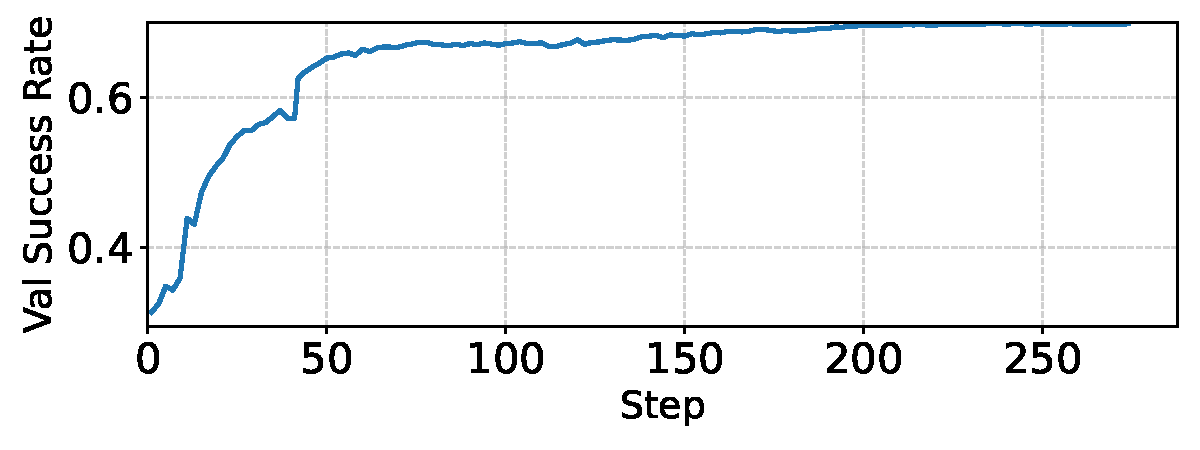
\includegraphics[width=0.5\linewidth]{figs/validation_trajectory_success_rate_fixed.pdf}
\caption{Validation trajectory success rate for the manager agent during RL fine-tuning (Hand-engineered-subgoal). The manager progressively adapts its subgoal proposals to compensate for employee imperfections, yielding steadily improving performance.}
%Validation trajectory success rate for the manager agent during training. (\red{Update this})}
\label{fig:valcurves}
\end{figure*}

\subsection{Agent Imperfections and Mechanisms to Overcome Them}

Trajectory failures arise when the agent does not complete the task before exceeding the allotted step limit, and these failures may occur at either the manager or employee level.  At the manager level, failures occur when the chosen subgoals are infeasible under the available command set or are misaligned with the final objective. Moreover, even when a subgoal is valid and achievable, execution may still fail if the employee is unable to complete it due to its own imperfections. 


At the employee level, failures typically stem from the agent's inability to distinguish between elementary items that must be gathered directly from the environment and intermediate items that must be crafted from them, from attempting to craft items that are infeasible given the current inventory, or from issuing invalid or unsupported crafting commands. We further observe that these errors most often arise when the employee attempts to complete a subgoal from an unfamiliar or abnormal inventory state, substantially different from those encountered during training. Such inventory states are themselves a consequence of imperfect execution of earlier subgoals, leading to situations where the agent collects irrelevant items or accumulates an excessive number of resources beyond what is needed. Notably, RL-based finetuning enables the manager to adapt to and compensate for these imperfections effectively.


\textbf{Manager Agent Accommodates Employee Imperfections.} 
To illustrate this, \Cref{tab:performance} (last row) reports a variant of our framework in which the employee is guided directly by a fixed sequence of achievable subgoals, without any manager adaptation. These subgoals are extracted from successful suboptimal trajectories in the validation set, using the same construction as the hand-engineered version (chosen in this study for its high interpretability). In principle, a perfect employee, trained on hand-engineered subgoals, could simply execute these subgoals sequentially to craft the ace item. However, without a manager to adjust the plan, this variant cannot recover when the employee fails to complete a subgoal in the sequence, resulting in a much lower success rate of 0.24. In contrast, the RL-finetuned manager adapts to such failures: when a proposed subgoal is not achieved (due to the employee's imperfect training), it receives no positive feedback and learns to propose alternative subgoals that the employee can successfully complete. Over time, the manager discovers easier, achievable subgoals that compensate for the employee's limitations, as also reflected in the steadily increasing success rates shown in \Cref{fig:valcurves}.

\begin{wrapfigure}{r}{0.45\linewidth}
    \centering
    \vspace{-15pt} % adjust if needed
    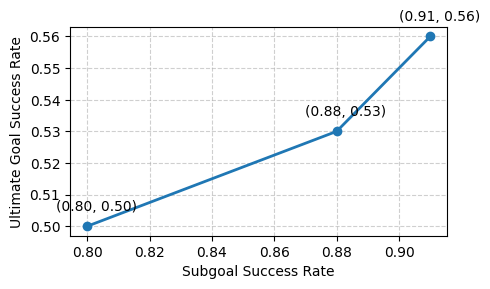
\includegraphics[width=\linewidth]{figs/SubgoalVSUltimateGoal}
    \caption{Subgoal vs. ultimate goal success rate in SCOPE.}
    \label{fig:SubgoalVSUltimateGoal}
    \vspace{-15pt} % adjust spacing below
\end{wrapfigure}


%\begin{figure}
%\centering
%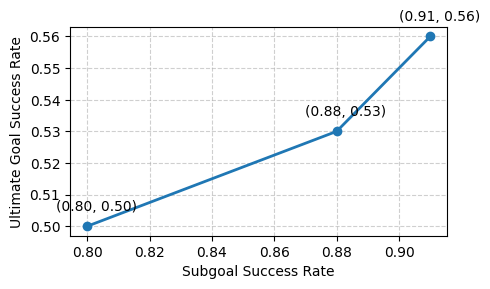
\includegraphics[width=0.45\linewidth]{figs/SubgoalVSUltimateGoal}
%\caption{Subgoal vs. ultimate goal success rate in SCOPE}
%\label{fig:SubgoalVSUltimateGoal}
%\end{figure}


\textbf{Stronger Employee Leads to Higher Success Rates.} While the manager can compensate for employee imperfections through RL finetuning, a stronger employee still substantially improves the final goal-achievement rate. \Cref{fig:SubgoalVSUltimateGoal} shows the relationship between subgoal success rate and ultimate goal success rate in SCOPE on the validation dataset, with weaker employee variants generated by evaluating partially trained checkpoints. As the figure illustrates, increases in subgoal success rate reliably translate into higher ultimate success, and this improvement accelerates when starting from a stronger employee. That is, higher subgoal success leads to disproportionately larger gains in overall goal completion. The effect is similar to compounding probabilities: the subgoal success rate applies repeatedly across steps, like a value raised to a power. When several subgoals must be achieved in sequence, even a small increase in subgoal reliability quickly compounds, resulting in much larger gains in final success.


\begin{figure*}
\centering
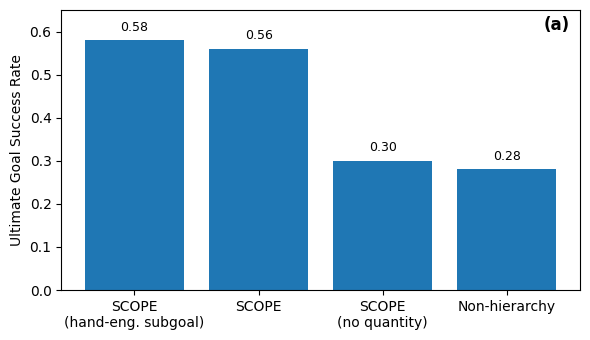
\includegraphics[width=0.48\linewidth]{figs/PerformanceVSSubgoalExplanability}~~~
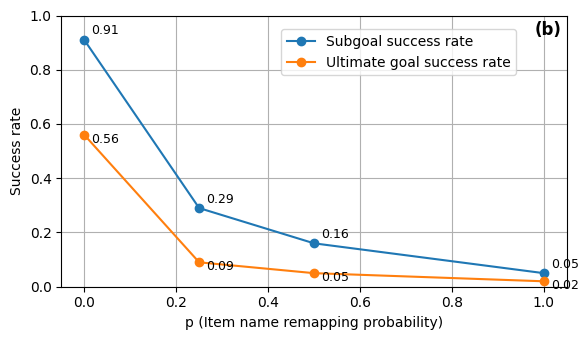
\includegraphics[width=0.48\linewidth]{figs/PerformanceVSItemNameRemapP}
\caption{Impact of subgoal quality on agent performance. (a) Performance vs.\ subgoal explainability (decreasing from left to right). (b) Effect of subgoals when their alignment with the environment is disrupted. Alignment is progressively broken by randomly remapping a proportion $p$ of item names in the LLM-generated subgoals, with $p \in \{0.0, 0.25, 0.5, 1.0\}$.}
\label{fig:PerformanceVSSubgoalExplanability}
\end{figure*}



\subsection{How Subgoals Help the Agent Complete the Game}
While the empirical study demonstrates that one-time LLM-generated subgoals enable SCOPE to surpass the LLM-driven hierarchical agent ADaPT, we now present additional ablations to analyze the source of this improvement more deeply.


\textbf{Impact of Subgoal Vagueness and Explainability.} As discussed in \cref{sec:impact_subopt_subgoal_performance}, LLM-generated subgoals are less explainable than hand-engineered ones, which likely contributes to the 2\% performance gap observed between SCOPE and the hand-engineered-subgoal variant. To further study how subgoal vagueness and explainability influence SCOPE’s performance, we include two additional variants, as shown in \cref{fig:PerformanceVSSubgoalExplanability}a. In SCOPE (no quantity), we remove the item-quantity information from LLM-generated subgoals, and a subgoal is considered satisfied once all listed item types have been collected at least once. Because this variant lacks quantity specifications, its subgoals are more ambiguous than those in standard SCOPE. We additionally include a limiting-case variant, Non-Hierarchical, which uses the same architecture and training setup as the employee agent (pretraining + RL fine-tuning) but is trained to pursue the final goal directly, without subgoals. In other words, the agent always conditions its decisions on the ultimate goal, rather than on any intermediate objectives. This represents the most vague scenario, as no subgoals are provided at all. As suggested by \cref{fig:PerformanceVSSubgoalExplanability}a, less interpretable and more vague subgoals make it harder for SCOPE to extract useful guidance for long-term planning, leading to a clear decline in ultimate goal success as explainability decreases.

\textbf{Effect of Decoupling Subgoals from Environment Outcomes.} To test whether subgoals contribute because they genuinely correspond to the environment outcomes, we design a mechanism that gradually breaks this connection by randomly remapping a ratio $p$ of item names in the LLM-generated subgoals. Specifically, when $p = 0$, subgoals are unchanged, which corresponds to the regular SCOPE; as $p$ increases, more item names are replaced by different ones, making the subgoals increasingly misleading; and when $p = 1.0$, all item names are remapped, meaning the subgoals no longer match the items that are actually needed in the environment. The remapping is sampled once and then fixed for both training and testing. We modify only the output of the subgoal-decomposition function, while leaving the subgoal-completion process unchanged, allowing us to degrade subgoal quality without altering the true task objective. This setup helps us understand how performance changes as the alignment between LLM-generated subgoals and environment outcomes is systematically removed, showing the extent to which correct subgoals are causally necessary for SCOPE's success. 


\cref{fig:PerformanceVSSubgoalExplanability}b shows how performance changes under different remapping probabilities $p$. When $p=0$, subgoals remain unchanged, and both subgoal and ultimate success rates are those of the regular SCOPE. As we increase $p$ and disrupt the correspondence between subgoals and the environment, performance drops rapidly. At $p=0.25$, success falls to 0.29 (subgoal) and 0.09 (ultimate), and continues to decrease as remapping increases, reaching only 0.05 and 0.02 at $p=1.0$. This sharp decline confirms that SCOPE relies critically on subgoals being causally aligned with the true environmental objectives. When this alignment is lost, both subgoal success and final goal completion collapse. Notably, even with only $25\%$ of item names remapped, the ultimate success rate drops to 0.09 -- substantially lower than the non-hierarchical agent's $0.28$, which operates without subgoals at all. This suggests that when subgoals lose alignment with the environment, they do not merely become unhelpful--they can actively mislead the agent. In contrast, earlier results show that vague but aligned subgoals (e.g., using LLM-generated subgoals instead of hand-engineered ones) remain helpful and degrade performance only mildly. It is the loss of alignment--not the loss of specificity--that is particularly harmful, underscoring that subgoals must remain causally grounded to benefit the agent. 















